\section{Context of the study}\label{sec:context}


This work is carried out in the context of the {\em Next-Generation Electrical Architecture (NGEA)} and {\em Next-Generation Electrical Architecture - step 2 (NGEAs)} projects, funded by Vinnova~\cite{Vinnova}. 
These projects are coordinated by Volvo Cars and involve the Chalmers University of Technology, some research centers in Sweden and many suppliers of the OEM, including Autoliv, Arccore, Combitech, Cybercom, Knowit, Prevas, \AA F-Technology, Semcom, and Qamcom. The projects aim to develop new software processes and proof of concepts to strengthen the competitiveness of the automotive industry in Sweden. The main objectives of the projects are to investigate (i) the transition of Volvo Cars towards continuous integration and deployment, (ii) new business models and innovative ways of working within the automotive ecosystem, and (iii) vehicles as part of system of systems. 
%Included in this project are sub projects or work packages that focus on 1) management, administration and business intelligence studies, 2) continuous deployment of architectural and development strategic viewpoints, and 3) automobiles as a system within an automotive software ecosystem \cite{Vinnova}. 
In this paper we mostly focus on point (ii) even though there will be some impact on point~(i). Since OEMs are becoming software companies, nowadays the automotive domain is increasingly attracting the attention of the software engineering community.  
%\todo{why relevant for ICSE?}

The automotive ecosystem consists of inter-organizational collaborations among automotive suppliers. It is characterized by relying on complex supplier networks and strong dependence on hardware and software development \cite{Knauss2014d}.
The current automotive industry is {\em closed}, with strict organizational boundaries, stiff processes, established business models and a straightforward value creation~\cite{ConnectedVehicle2012}.


Nowadays, a vehicle is a {\em driving software package} as compared to the vehicles of not even ten years ago. J\"orgen M\"ossinger, VP for automotive systems integration at Bosch, said: ``Electronics and especially software are the main sources of automotive innovation today."~\cite{Mossinger2010SoftwareAutomotive}. The Boston Consulting Group estimates that the total costs of electronic parts will rise from 20\% of the value in a typical car in 2004 to 40\% in 2015. Software, instead of hardware, has become the differentiating factor% of products
~\cite{ConnectedVehicle2012,hbr2015hardwaresoftware,Mossinger2010SoftwareAutomotive,Broy:2006:CAS:1134285.1134292} %. In the past, hardware was the differentiator 
between companies and their products. This evolution of the automotive industry, illustrated by the exponential increase of software, creates new challenges regarding software integration, development, deployment, and maintenance. Therefore, its development needs to support the related integration and evolution of time~\cite{Broy:2006:CAS:1134285.1134292,qualman2009socialnomics,JansenTale2009}. The increasing amount of stakeholders involved in the software development projects imposes additional challenges to the architecture teams, as the development and design literally cannot be controlled, or even understood, in detail by a single group any more. 

The stakeholders in the automotive ecosystem are classified as OEMs (e.g. Volvo Cars) and its suppliers (Tier-1 and Tier-2). In general the OEM is the coordinator and platform owner in the automotive ecosystem~\cite{KS15}. Tier-1 suppliers are considered direct suppliers to OEM and Tier-2 companies are a second level of suppliers, indirect to the OEM and directly connected to Tier-1. % and vice versa, hence, indirect to the OEM. \todo{is this relevant+understandable by ICSE readers?}

\begin{figure}[htb]
\vspace{-.2cm}
\centering
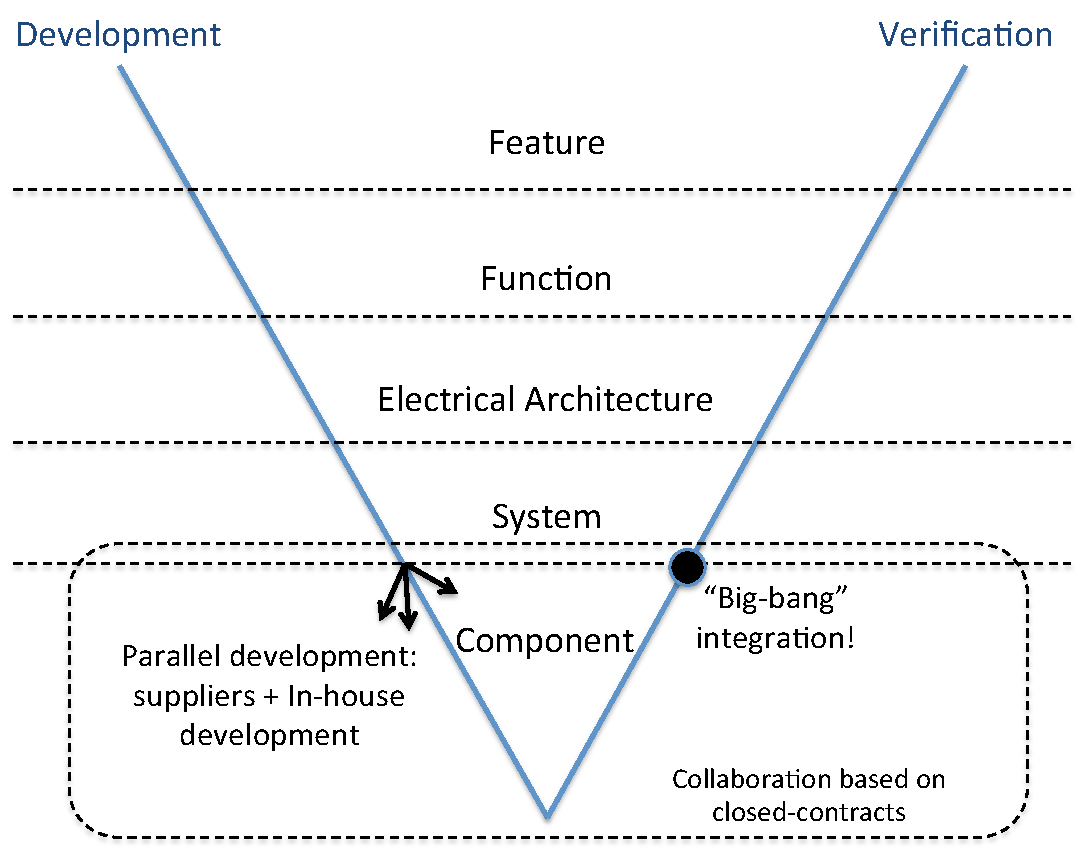
\includegraphics[width=\columnwidth]{figure/Closed-contract-collaboration.pdf}
\vspace{-.2cm}
\caption{Collaboration based on contracts}
\label{fig:closedContractCollaboration}
\vspace{-.2cm}
\end{figure}

Therefore, OEMs experience heavy reliance on external developers and subcontractors; this complicates coordination throughout the entire development process. Expensive communication and coordination delays during integration are results of outsourcing significant parts of development to suppliers. %This form of exponentially growing feature content severely complicates ``big-bang" integration~\cite{Eklund2012}. The development is inevitably parallelized; this obviously also holds for the large amount of externally developed software, which is integrated as black-box functionality~\cite{Patrizio2016AAF_Chalmers,Broy2009AAF_TUM,Broy:2006:CAS:1134285.1134292}. 

As shown in Figure~\ref{fig:closedContractCollaboration} the software engineering process follows the V-model, with the development on the left-hand side and verification on the right-hand side. The development at the level of components is parallelized among the different suppliers, and internal in-house development. The degree of parallelism can easily reach level 50 (i.e. 50 parallel developments). Once the collaboration between the OEM and its suppliers is regulated by contract, the parallel developments represented in Figure~\ref{fig:closedContractCollaboration} start by signing a contract and then after months the large amount of externally developed software come back to the OEM and it is integrated as black-box functionality~\cite{Broy:2006:CAS:1134285.1134292}. 
%the produced ECUs will be provided back to the OEM after some months with few communication during the production period.
This leads to the above mentioned ``big bang" integration~\cite{Eklund2012}. %: the developed Electronic Control Units (ECUs) (which include both hardware and software) come back to the OEM and integration starts. 
It is at this stage that many misunderstandings, conflicting interpretations, wrong assumptions, etc. are discovered.
It is easy to understand that contract relations between the OEM and the suppliers can slow down the system-wide CI\&D.  %\todo{this last statement is disconnected from the rest of the story: miss the link between the mentioned integration problems and closed contracts}

%The collaboration between the stakeholders in the ecosystem needs to improve the software quality and provide faster, cheaper, and more predictable development~\cite{herbsleb2016IntelligentTransparent}. 
%
%This implies that the automotive (software) industry must identify how this new scenario\todo{what is the new scenario?} can be supported at best when an ecosystem of organizations collaborates.
%
%\todo{there is a gap between these two paragraphs: collaboration should be supported by new tools, like views and associated viewpoints to communicate the right architectural knowledge, etc.}
%
%These considerations motivate the need of considering new types of viewpoints and views\todo{add citation} from the perspective of specific system concerns, which are relevant for one or more stakeholders collaborating in the automotive ecosystem. Because of this, it is necessary for members of this ecosystem to agree on a common way of structuring\todo{what do you mean? structuring what?} in order to increase overall efficiency within the ecosystem \cite{Patrizio2016AAF_Chalmers,Broy2009AAF_TUM,Broy:2006:CAS:1134285.1134292}. An essential technical problem to solve for this vision is the establishment of standards for interoperability among IPs, both software and hardware, and tools \cite{Broy:2006:CAS:1134285.1134292}. ``Establishing and evolving ecosystems of different partner types might ultimately decide which companies win a market." \cite{Bosch2016Ecosystem}. First attempts, such as AUTOSAR \cite{acm2008autosar} and the Automotive Architecture Framework (AAF) \cite{Patrizio2016AAF_Chalmers,Broy2009AAF_TUM} are being developed. However, researchers and practitioners both identified the need for further research on this emerging type of software ecosystems.
%
